

\tikzset{every picture/.style={line width=0.75pt}} %set default line width to 0.75pt        

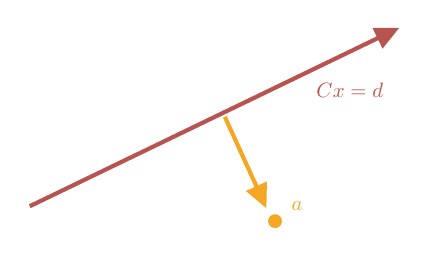
\begin{tikzpicture}[x=0.75pt,y=0.75pt,yscale=-1,xscale=1]
%uncomment if require: \path (0,300); %set diagram left start at 0, and has height of 300

%Straight Lines [id:da9999289567232588] 
\draw [color={rgb, 255:red, 184; green, 84; blue, 80 }  ,draw opacity=1 ][fill={rgb, 255:red, 184; green, 84; blue, 80 }  ,fill opacity=1 ][line width=1.5]    (241,170.65) -- (415.4,86.41) ;
\draw [shift={(419,84.67)}, rotate = 154.22] [fill={rgb, 255:red, 184; green, 84; blue, 80 }  ,fill opacity=1 ][line width=0.08]  [draw opacity=0] (11.61,-5.58) -- (0,0) -- (11.61,5.58) -- cycle    ;
%Shape: Circle [id:dp5553159381717454] 
\draw  [color={rgb, 255:red, 245; green, 166; blue, 35 }  ,draw opacity=1 ][fill={rgb, 255:red, 245; green, 166; blue, 35 }  ,fill opacity=1 ] (356.35,177.82) .. controls (356.35,176.26) and (357.62,175) .. (359.18,175) .. controls (360.74,175) and (362,176.26) .. (362,177.82) .. controls (362,179.38) and (360.74,180.65) .. (359.18,180.65) .. controls (357.62,180.65) and (356.35,179.38) .. (356.35,177.82) -- cycle ;
%Straight Lines [id:da5135858807849654] 
\draw [color={rgb, 255:red, 245; green, 166; blue, 35 }  ,draw opacity=1 ][fill={rgb, 255:red, 184; green, 84; blue, 80 }  ,fill opacity=1 ][line width=1.5]    (335,127.57) -- (353.34,167.93) ;
\draw [shift={(355,171.57)}, rotate = 245.56] [fill={rgb, 255:red, 245; green, 166; blue, 35 }  ,fill opacity=1 ][line width=0.08]  [draw opacity=0] (11.61,-5.58) -- (0,0) -- (11.61,5.58) -- cycle    ;

% Text Node
\draw (378,110) node [anchor=north west][inner sep=0.75pt]  [color={rgb, 255:red, 184; green, 84; blue, 80 }  ,opacity=1 ,xscale=0.75,yscale=0.75]  {$Cx=d$};
% Text Node
\draw (366,167.4) node [anchor=north west][inner sep=0.75pt]  [xscale=0.75,yscale=0.75]  {$\textcolor[rgb]{0.96,0.65,0.14}{a}$};


\end{tikzpicture}